\PassOptionsToPackage{table}{xcolor}
\documentclass[aspectratio=169]{beamer}\usepackage[utf8]{inputenc}
\usepackage{lmodern}
\usepackage[english]{babel}
\usepackage{color}
\usepackage{amsmath,mathtools}
\usepackage{booktabs}
\usepackage{mathptmx}
\usepackage[11pt]{moresize}
\usepackage{hyperref}
\usepackage{commath}
\usepackage{bm}
\usepackage{subfigure}
\usepackage{siunitx}

\setbeamertemplate{navigation symbols}{}
\setbeamersize{text margin left=5mm,text margin right=5mm}
\setbeamertemplate{caption}[numbered]
\addtobeamertemplate{navigation symbols}{}{
\usebeamerfont{footline}
\usebeamercolor[fg]{footline}
\hspace{1em}
\insertframenumber/\inserttotalframenumber}

\newcommand{\R}{\mathbb{R}}
\newcommand{\E}{\mathbb{E}}
\newcommand{\N}{\mathbb{N}}
\newcommand{\Z}{\mathbb{Z}}
\newcommand{\V}{\mathbb{V}}
\newcommand{\Q}{\mathbb{Q}}
\newcommand{\K}{\mathbb{K}}
\newcommand{\C}{\mathbb{C}}
\newcommand{\T}{\mathbb{T}}
\newcommand{\I}{\mathbb{I}}
\DeclareMathOperator{\sign}{sign}

\title{Initial Guess}
\subtitle{Renzo Miguel Caballero Rosas}

\begin{document}

\begin{frame}
\titlepage
{\tiny Note: We compute the following results using \textbf{errorVsForecast.m} and \textbf{plot\_epsilon.m}.}
\end{frame}


%\setbeamercolor{background canvas}{bg=white!10}
%\begin{frame}\frametitle{Discrete approximation}
%
%We consider the transition $\Delta V_i=V_{i+1}-V_i$ with $\Delta t=t_{i+1}-t_i$, and we approximate the SDE by its Euler–Maruyama scheme for $t\in\left\{t_i,t_{i+1}\right\}$:
%\begin{equation*}
%\begin{cases}
%{\color{blue}V(t_{i+1})}&={\color{blue}V(t_i)-\theta_{t_i}V(t_i)\Delta t}+\sqrt{2\theta_0\alpha(V(t_i)+p_i)(1-V(t_i)-p_i)\Delta t}\Delta W\\
%V(t_i)&=V_i.
%\end{cases}
%\end{equation*}
%Then, ${\color{blue}V_{i+1}-V_{i}(1-\theta_{t_i}\Delta	t)}$ is a random variable with Gaussian distribution, zero mean and variance
%\begin{equation*}
%\sigma^2_i=2\theta_0\alpha(V_i+p_i)(1-V_i-p_i)\Delta t.
%\end{equation*}
%The approximation becomes better as $\Delta t$ becomes smaller.
%\end{frame}
%
%
%\setbeamercolor{background canvas}{bg=white!10}
%\begin{frame}\frametitle{Discrete approximation}
%
%Now, we consider a total of $n$ transitions $\{\Delta V_i\}_{i=1}^n$ with the corresponding forecasts $\{p_i\}_{i=1}^n$. Then, we can approximate the variance using means:
%\begin{equation*}
%\frac{1}{n}\sum_{i=1}^n\left(V_{i+1}-V_i(1-\theta_{t_i}\Delta t)\right)^2\approx\frac{1}{n}\sum_{i=1}^n\left[2\theta_0\alpha(V_i+p_i)(1-V_i-p_i)\Delta t\right],
%\end{equation*}
%from where we can deduce
%\begin{equation}
%\frac{\sum_{i=1}^n\left(V_{i+1}-V_i(1-\theta_{t_i}\Delta t)\right)^2}{2\Delta t\sum_{i=1}^n(V_i+p_i)(1-V_i-p_i)}\approx\theta_0\alpha.
%\label{Eq-1}
%\end{equation}
%
%\end{frame}


\setbeamercolor{background canvas}{bg=white!20}
\begin{frame}\frametitle{Boundedness of $\theta_t$ (we define $\theta_t^\epsilon$)}\label{theta_t}
To guarantee an unique solution for the process $X_t$, we need boundedness in $\theta_t$ for $t\in[0,T]$. For our definition
\begin{equation}
\theta_t=\max\left(\theta_0,\frac{\alpha\theta_0+|2\dot{p}_t|}{2\min(1-p_t,p_t)}\right),
\label{Eq-6}
\end{equation}
we do not have a bound for $\theta_t$ if $p_t\to0^+$ or $p_t\to1^-$.
However, if we ensure that $p_t\in[\epsilon,1-\epsilon]$ for some $0<\epsilon<\frac{1}{2}$ and all $t\in[0,T]$, then $\theta_t<M(\epsilon)<\infty$ for all $t\in[0,T]$.\\
So, we define the corrected forecast
\begin{equation}
p_t^\epsilon=\begin{cases}
\epsilon\quad&\text{if}\quad p_t<\epsilon\\
p_t\quad&\text{if}\quad\epsilon\leq p_t<1-\epsilon\\
1-\epsilon\quad&\text{if}\quad p_t\geq1-\epsilon,
\end{cases}
\label{Eq-5}
\end{equation}
and the corrected (and bounded) drift coefficient
\begin{equation}
\theta_t^\epsilon=\max\left(\theta_0,\frac{\alpha\theta_0+2|\dot{p}_t^\epsilon|}{2\min(1-p_t^\epsilon,p_t^\epsilon)}\right).
\label{Eq-11}
\end{equation}

\end{frame}


\setbeamercolor{background canvas}{bg=white!20}
\begin{frame}\frametitle{Boundedness of $\theta_t$ (we define $\theta_t^\epsilon$)}

Using our new definition $\theta_t^\epsilon$ in the drift of our SDE:
\begin{itemize}

\item We guarantee existence and uniqueness of the solution, and that $X_t\in]0,1[$ for all $t\in[0,1]$.
\item As $X_t\in]0,1[$, the Lamperti transform is well defined for all $t\in[0,T]$ and we can use It\^o's lemma to compute the SDE for the transformed process.

\end{itemize}

\end{frame}


\setbeamercolor{background canvas}{bg=white!20}
\begin{frame}\frametitle{Least square minimization (LSM)}\label{S1}
{\small
\begin{columns}[c]

\column{.6\textwidth}
We consider the transition $\Delta V_i=V_{i+1}-V_i$ with $\Delta t=t_{i+1}-t_i$. $(V_{i+1}|V_i)$ is a random variable which conditional mean can be approximated by the solution of the system
\begin{equation*}
\begin{cases}
\dif \E\left[V\right]&=-\theta_t^\epsilon\E\left[V\right]\dif t\\
\E\left[V(t_i)\right]&=V_i,
\end{cases}
\end{equation*}
evaluated in $t_{i+1}$ (i.e., $\E\left[V(t_{i+1})\right]$). Then, the random variable $(V_{i+1}-\E\left[V(t_{i+1})\right])$ has approximately zero mean.

\column{.3\textwidth}
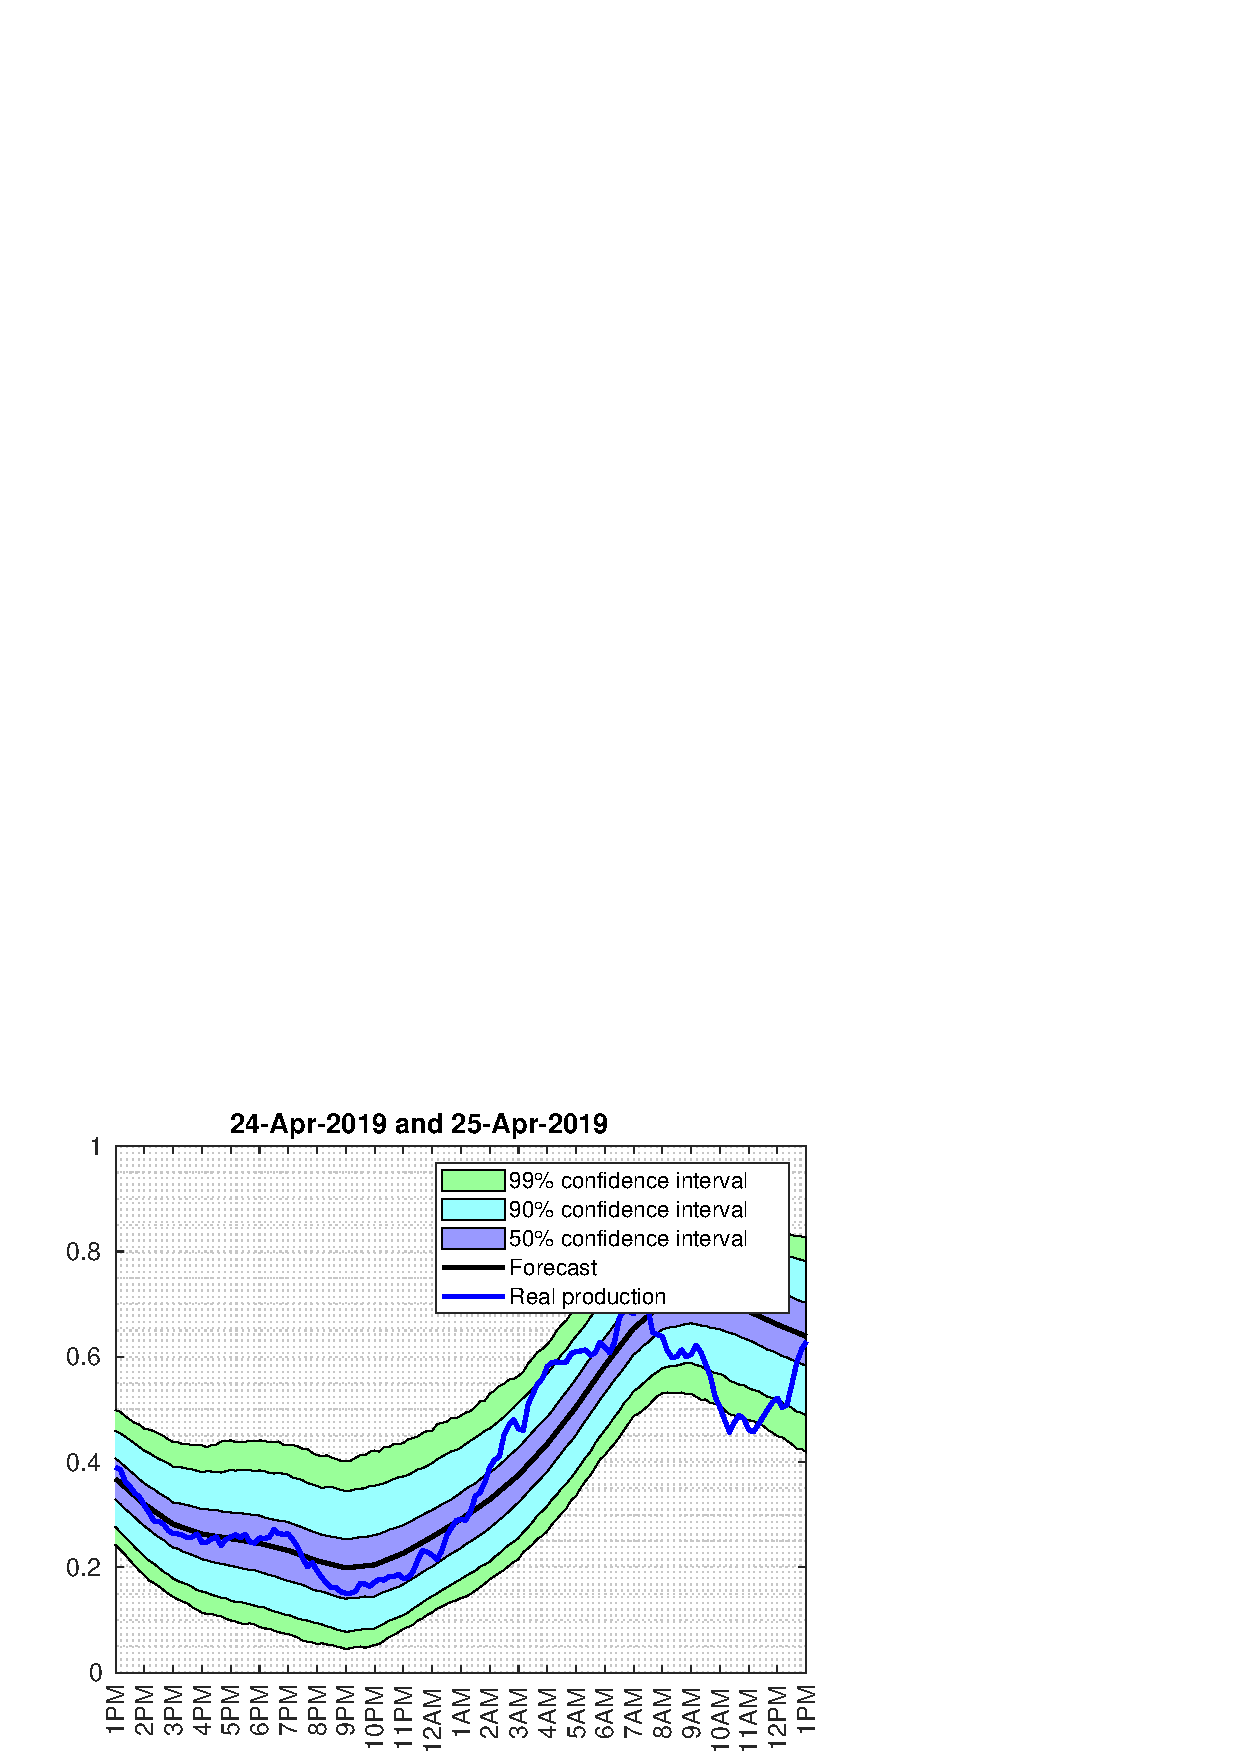
\includegraphics[width=0.7\columnwidth]{1.jpg}

\end{columns}}
\quad\\
\quad\\
If we assume that $\theta_t^\epsilon=\alert{c}\in\R^+$ for all $t\in[t_i,t_{i+1}]$, then $\E\left[V(t_{i+1})\right]=V_ie^{-\alert{c}\Delta t}$. If we have a total of $n$ transitions, we can write the regression problem for the conditional mean with $L^2$ loss function as
\begin{equation}
\alert{c}^*\approx\arg\min_{\alert{c}\geq0}\left[\sum_{i=1}^n\left(V_{i+1}-\E\left[V(t_{i+1})\right]\right)^2\right]=\arg\min_{\alert{c}\geq0}\left[\sum_{i=1}^n\left(V_{i+1}-V_ie^{-\alert{c}\Delta t}\right)^2\right].
\label{Eq-1}
\end{equation}

\end{frame}


\setbeamercolor{background canvas}{bg=white!20}
\begin{frame}\frametitle{Least square minimization (we are assuming $\theta_t^\epsilon=\alert{c}\in\R^+$)}

We take the first order approximation w.r.t. $\alert{c}$
\begin{equation*}
e^{-\alert{c}\Delta t}=1-\alert{c}\Delta t+\mathcal{O}\left((\alert{c}\Delta t)^2\right),
\end{equation*}
and introduce it in equation ({\color{blue}\ref{Eq-1}}). We get
\begin{equation}
\alert{c}^*\approx\arg\min_{\alert{c}\geq0}\underbrace{\left[\sum_{i=1}^n\left(V_{i+1}-V_i(1-\alert{c}\Delta t)\right)^2\right]}_{:=f(\alert{c})}.
\label{Eq-3}
\end{equation}
As $f(\alert{c})$ is convex in $\alert{c}$, solving ({\color{blue}\ref{Eq-3}}) (finding $\alert{c}^*$) is equivalent to solving
\begin{equation}
\frac{\partial f}{\partial\alert{c}}(\alert{c}^{**})=0,
\label{Eq-9}
\end{equation}
and choosing $\alert{c}^*=\max\{0,\alert{c}^{**}\}$.

\end{frame}


\setbeamercolor{background canvas}{bg=white!20}
\begin{frame}\frametitle{Least square minimization (we are assuming $\theta_t^\epsilon=\alert{c}\in\R^+$)}\label{QMM}

\begin{equation*}
\begin{split}
\frac{\partial f}{\partial\alert{c}}&=\sum_{i=1}^n2(-V_i)(-\Delta t)(V_{i+1}-V_i(1-\theta_0\Delta t))\\
&=\sum_{i=1}^n2V_i\Delta t(V_{i+1}-V_i(1-\alert{c}\Delta t))\\
&=\sum_{i=1}^n2V_{i+1}V_i\Delta t-2V_i^2\Delta t+2V_i^2\Delta t^2\alert{c}.
\end{split}
\end{equation*}
Then, $\alert{c}^{**}$ satisfies
\begin{equation}
\alert{c}^{**}\approx\frac{\sum_{i=1}^nV_i(V_i-V_{i+1})}{\Delta t\cdot\sum_{i=1}^n(V_i)^2}.
\label{Eq-4}
\end{equation}
Notice that $\alert{c}^{**}$ has dimension $\mathbf{time}^{-1}$.

\end{frame}


\setbeamercolor{background canvas}{bg=white!10}
\begin{frame}\frametitle{Quadratic variation}\label{QV}

We approximate the SDE by its E-M scheme. In particular, we approximate the It\^o quadratic variation with the discrete one:
\begin{itemize}

\item It\^o process quadratic variation: $[V]_t=\int_0^t\sigma_s^2\dif s$.
\item Discrete process quadratic variation: $[V]_t=\sum_{0<s\leq t}(\Delta V_s)^2$.

\end{itemize}
\quad\\
\quad\\
Then, considering $\Delta t$ the time between measurements, we approximate:
\begin{equation}
\theta_0^*\alpha^*\approx\frac{\sum_{i=1}^n(\Delta V_i)^2}{2\Delta t\sum_{i=1}^n(V_i+p_i)(1-V_i-p_i)}.
\label{Eq-2}
\end{equation}

\end{frame}


\setbeamercolor{background canvas}{bg=white!20}
\begin{frame}\frametitle{Estimation of $(\theta_0,\alpha,\epsilon)$}

In slide ({\color{blue}\ref{theta_t}}) we defined the parameter $\epsilon$ which has as only condition $0<\epsilon<\frac{1}{2}$. We want to estimate the set of parameters $(\theta_0,\alpha,\epsilon)$, we call to the estimations $(\theta_0^*,\alpha^*,\epsilon^*)$.\\
\quad\\
Recall from slide ({\color{blue}\ref{S1}}) that, to use the LSM estimation, we assume $\theta_t^\epsilon=\alert{c}\in\R^+$. Recall also our definition for $\theta_t^\epsilon$ (equation ({\color{blue}\ref{Eq-11}})):
\begin{equation*}
\theta_t^\epsilon=\max\left(\theta_0,\frac{\alpha\theta_0+2|\dot{p}_t^\epsilon|}{2\min(1-p_t^\epsilon,p_t^\epsilon)}\right).
\end{equation*}
Fixed $\epsilon$, we call $\mathcal{V}=\{\Delta V_i^\epsilon\}_{i=1}^n$ to the set of $n$ error transitions where for each measurement $X_i$, we have that $V_i=X_i-p_i^\epsilon$. $\mathcal{P}=\{p_i^\epsilon\}_{i=1}^n$ is the corresponding set of forecasts.\\
Now, if we also fix $\theta_0$ and $\alpha$, we can define the set of indexes $\mathbf{I}=\{i\in\{1,\dots,n\}:\text{ the LSM estimation will estimate }\theta_0\}$ and $\mathbf{J}=\left\{j\in\{1,\dots,n\}:\text{ the LSM estimation will estimate }\frac{\theta_0\alpha}{\epsilon}\right\}$.

\end{frame}


\setbeamercolor{background canvas}{bg=white!20}
\begin{frame}\frametitle{Estimation of $(\theta_0,\alpha,\epsilon)$}\label{Slide:Defs}

From the definition of $\theta_t^\epsilon$: We have that for $\epsilon<<1$, and $p_t=\epsilon$ or $p_t=1-\epsilon$, the approximation $\theta^\epsilon_t\approx\frac{\theta_0\alpha}{\epsilon}$ holds. Then, for $\epsilon$ small enough, $\mathbf{J}$ can be approximated by $$\mathbf{J}\approx\tilde{\mathbf{J}}=\{j\in\{1,\dots,n\}:p_j^\epsilon\in\{\epsilon,1-\epsilon\}\}.$$
Now, coming back to the definition of $\theta_t^\epsilon$, we have that it is more likely that $\theta_t^\epsilon=\theta_0$ if $p_t^\epsilon\approx\frac{1}{2}$. Then, we can approximate $\mathbf{I}$ by $$\mathbf{I}\approx\tilde{\mathbf{I}}=\left\{i\in\{1,\dots,n\}:p_i\in(\gamma,1-\gamma)\right\},\ \gamma\approx\frac{1}{2},\ \gamma<\frac{1}{2}.$$

\end{frame}


\setbeamercolor{background canvas}{bg=white!20}
\begin{frame}\frametitle{Estimation of $(\theta_0,\alpha,\epsilon)$: $\theta_0^*$}

\begin{figure}[ht!]
\centering
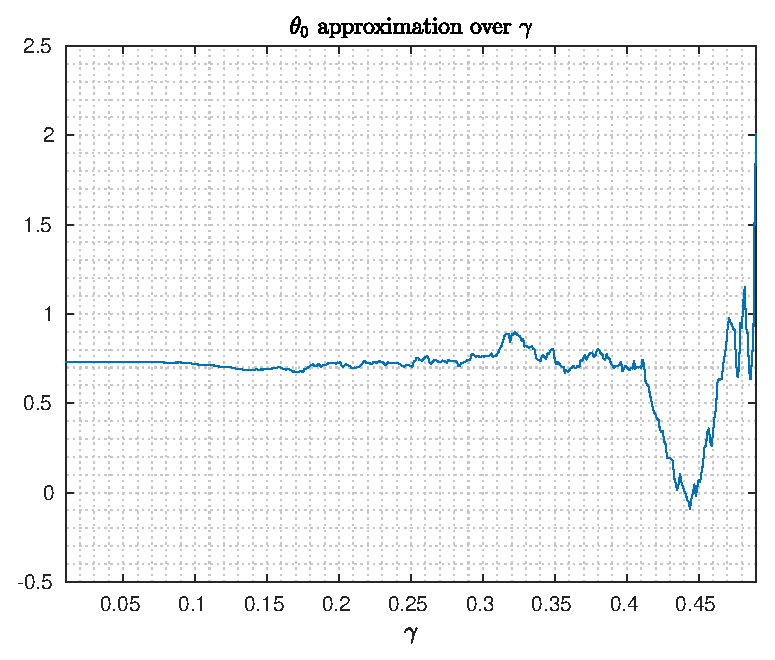
\includegraphics[width=0.4\textwidth]{../../MATLAB_Files/Results/epsilon/theta_0.eps}\quad\quad
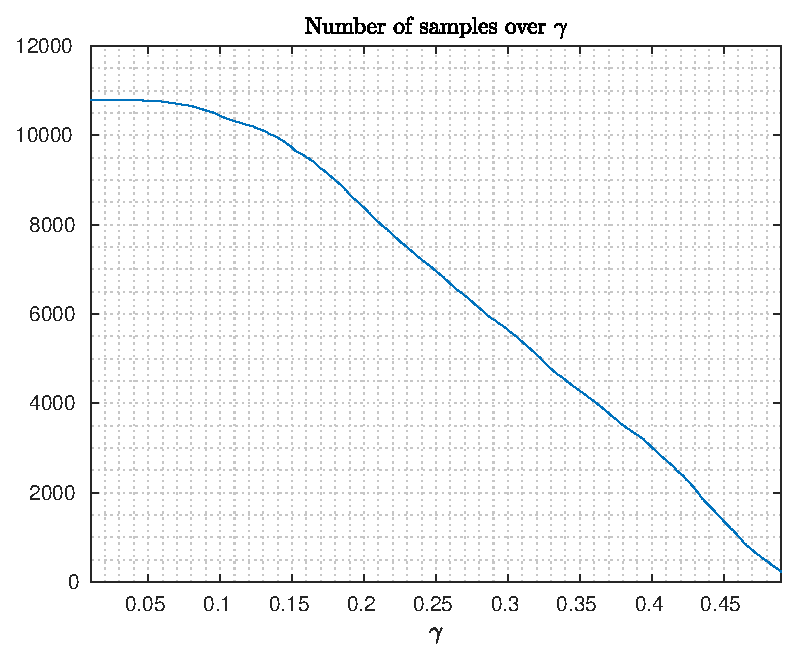
\includegraphics[width=0.4\textwidth]{../../MATLAB_Files/Results/epsilon/num_over_eps_t0.eps}
\end{figure}

In slide ({\color{blue}\ref{Slide:Defs}}), we showed that for $\gamma\approx\frac{1}{2}$, the LSM estimation using indetex from $\tilde{\mathbf{I}}$ is an estimator for $\theta_0$. On the left, we can see $\theta_0^*$ as a function of $\gamma$. The choose ${\color{orange}\theta_0^*\approx1.25}$ seems reasonable from the plot.


\end{frame}


\setbeamercolor{background canvas}{bg=white!20}
\begin{frame}\frametitle{Estimation of $(\theta_0,\alpha,\epsilon)$: $\theta_0^*\alpha^*$ and $\alpha^*$}

Recall the quadratic variation estimator ({\color{blue}\ref{Eq-2}}) from slide ({\color{blue}\ref{QV}}). It uses all the transitions $\mathcal{V}$ and estimated the product $\theta_0\alpha$.\\
\quad\\
We get ${\color{orange}\theta_0^*\alpha^*\approx0.10}$, from where we calculate ${\color{orange}\alpha^*\approx0.08}$.

\end{frame}


\setbeamercolor{background canvas}{bg=white!20}
\begin{frame}\frametitle{Estimation of $(\theta_0,\alpha,\epsilon)$: $\epsilon^*$}

As we have an approximated value for $\theta_0\alpha$, if we can estimate $\frac{\theta_0\alpha}{\epsilon}$, then we can estimate $\epsilon$. In slide ({\color{blue}\ref{Slide:Defs}}), we showed that for $\epsilon<<1$, the LSM estimation using indexes from $\tilde{\mathbf{J}}$ is an estimator for $\frac{\theta_0\alpha}{\epsilon}=:k$.\\
\quad\\
However, which values of $\epsilon$ satisfies $\epsilon<<1$? We choose an initial guess for $\epsilon$ (call it $\epsilon_0$), and iterating we aim to converge to some local minimum. We proceed with the following steps:

\begin{itemize}

\item We sample $\epsilon_0$ from $\mathcal{U}[0.01,0.1]$ and load $\epsilon\gets\epsilon_0$.
\item We create $\tilde{\mathbf{J}}$ and use the LSM estimation to find $k$. If $k<\theta_0^*$, then the assumption $\theta_t^\epsilon=\alert{c}\in\R^+$ is wrong and we reduce the value of $\epsilon$, i.e., $\epsilon\gets\epsilon*0.999$. If $k\geq\theta_0^*$, we load $\epsilon\gets\frac{\theta_0^*\alpha^*}{k}$ (we allow a maximum relative change of 1\%). We repeat this step *100 times*.
\item We repeat steps 1 and 2 *500 times*. After, we plot the results.

\end{itemize}

\end{frame}


%\setbeamercolor{background canvas}{bg=white!10}
\begin{frame}\frametitle{Estimation of $(\theta_0,\alpha,\epsilon)$: $\epsilon^*$}

\begin{columns}

\column{.45\textwidth}
We can see that we converge to four different local minimums.

\column{.45\textwidth}
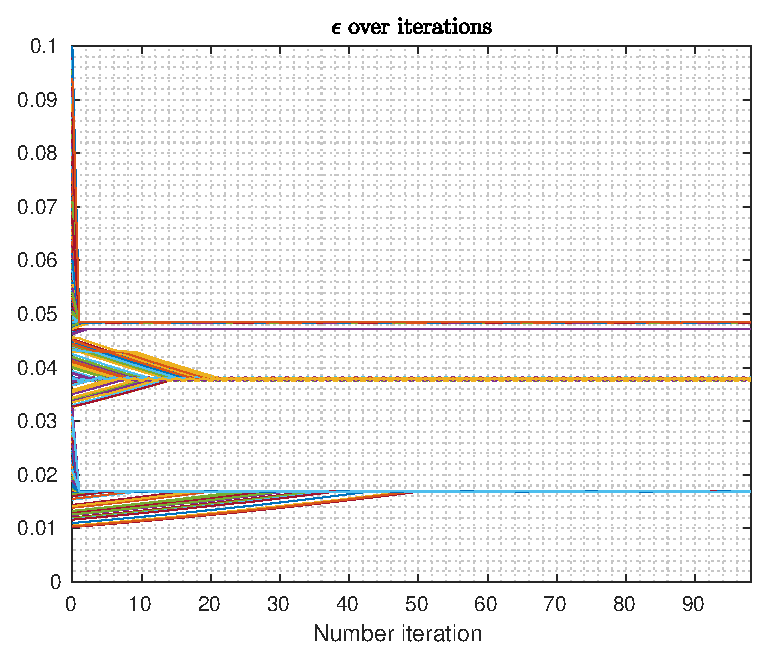
\includegraphics[width=1\textwidth]{../../MATLAB_Files/Results/epsilon/epsilon.eps}
\end{columns}

\end{frame}


%\setbeamercolor{background canvas}{bg=white!10}
\begin{frame}\frametitle{Estimation of $(\theta_0,\alpha,\epsilon)$: $\epsilon^*$}

\begin{columns}

\column{.45\textwidth}
This is the value of $k$ over iterations. When $k<\theta^*_0$, we assume that the estimation and repeat the iteration step.

\column{.45\textwidth}
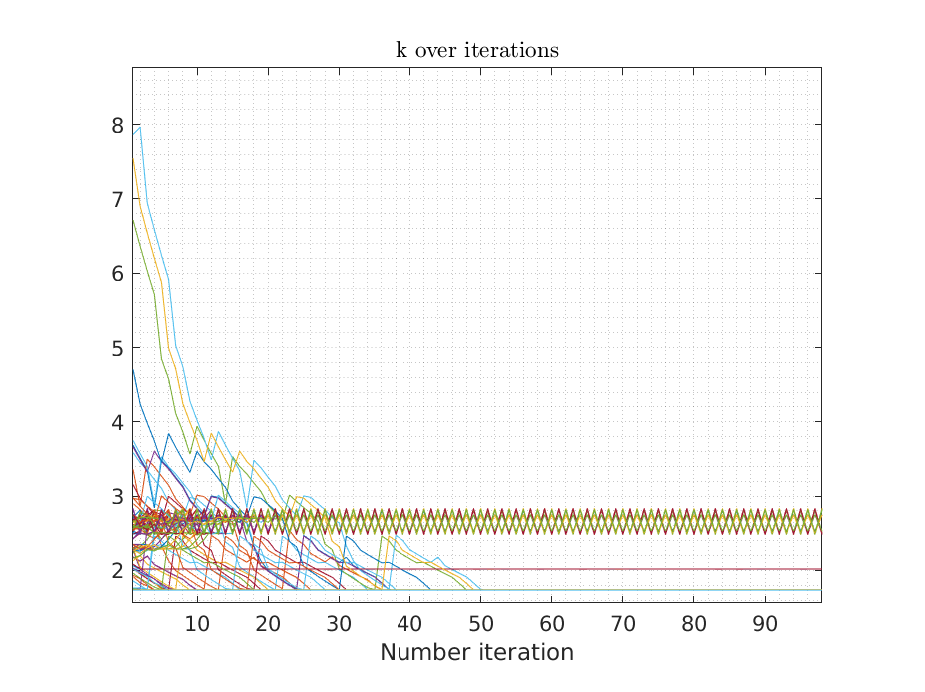
\includegraphics[width=1.1\textwidth]{../../MATLAB_Files/Results/epsilon/theta_t.eps}
\end{columns}

\end{frame}


%\setbeamercolor{background canvas}{bg=white!10}
\begin{frame}\frametitle{Estimation of $(\theta_0,\alpha,\epsilon)$: $\epsilon^*$}

\begin{columns}

\column{.45\textwidth}
In this plot, we can see the minimum of the normalized value function ({\color{blue}\ref{Eq-1}}) over $\epsilon$. We normalize it with respect to the number of elements of $\tilde{\mathbf{J}}$.
\begin{itemize}

\item Using fixed $k$: As $k<\theta^*_0$ has not sense, when we get that condition we set $k\gets\theta^*_0$, and evaluate the value function in $k$.
\item Analytical optimal value function.
\item Numerical optimal value function.

\end{itemize}
We can see that all plots almost coincide. We choose ${\color{orange}\epsilon^*\approx0.018}$.

\column{.45\textwidth}
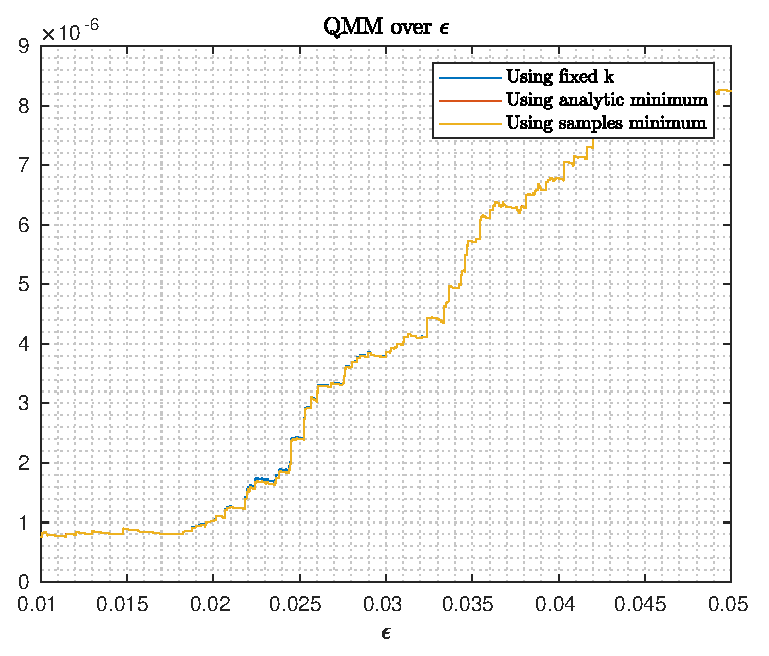
\includegraphics[width=1\textwidth]{../../MATLAB_Files/Results/epsilon/QMM.eps}
\end{columns}

\end{frame}


%\setbeamercolor{background canvas}{bg=white!10}
\begin{frame}\frametitle{Estimation of $(\theta_0,\alpha,\epsilon)$: $\epsilon^*$}

\begin{columns}

\column{.45\textwidth}
When we get $k<\theta^*_0$, we set $k\gets\theta_0^*$.

\column{.45\textwidth}
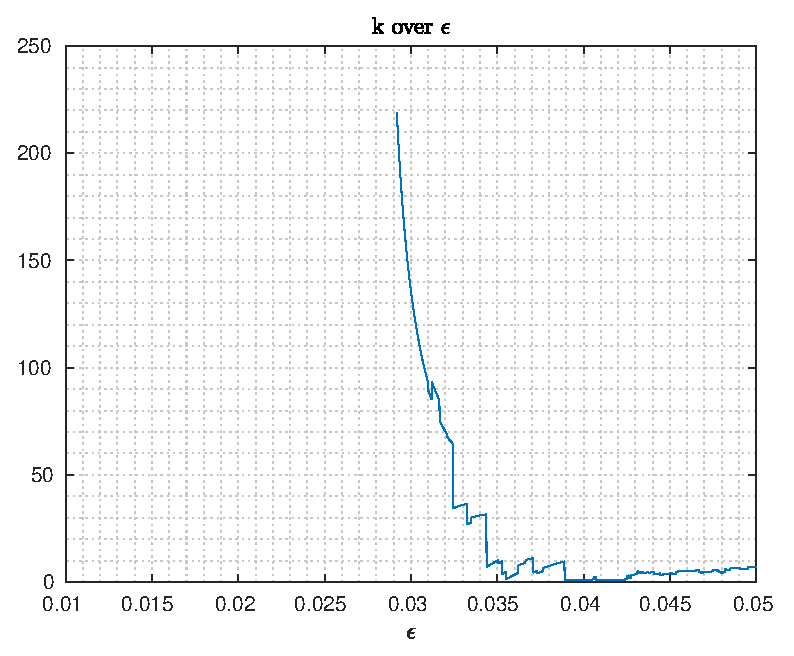
\includegraphics[width=1\textwidth]{../../MATLAB_Files/Results/epsilon/theta_over_eps.eps}
\end{columns}

\end{frame}



%\setbeamercolor{background canvas}{bg=white!10}
\begin{frame}\frametitle{Estimation of $(\theta_0,\alpha,\epsilon)$: $\epsilon^*$}

\begin{columns}

\column{.45\textwidth}
Number of elements in $\tilde{\mathbf{J}}$ as a function of $\epsilon$.

\column{.45\textwidth}
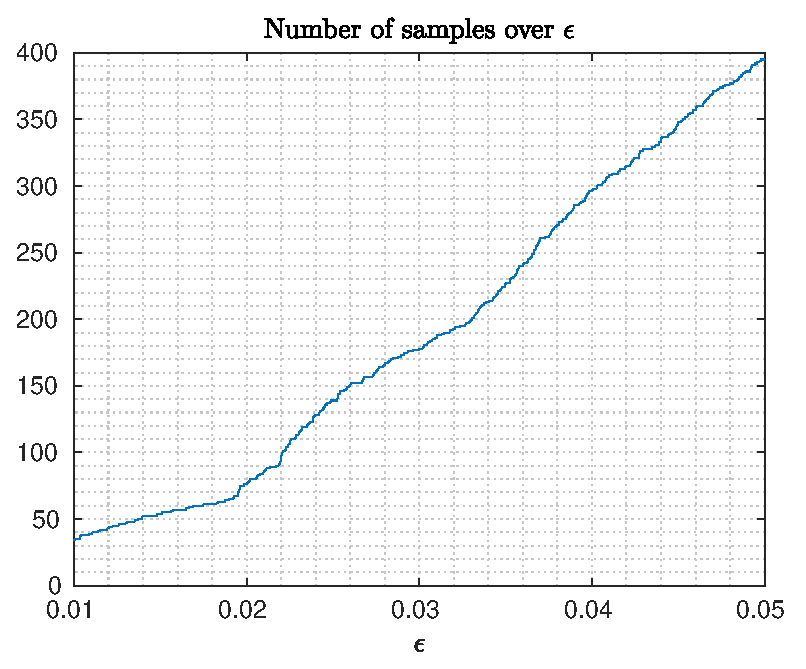
\includegraphics[width=1\textwidth]{../../MATLAB_Files/Results/epsilon/num_over_eps.eps}
\end{columns}

\end{frame}


\setbeamercolor{background canvas}{bg=white!10}
\begin{frame}\frametitle{Extra: Interesting data processing}

\begin{figure}[ht!]
\centering
\includegraphics[width=0.4\textwidth]{../../../Python/Represas_Data_2/Wind_Data/someResults/final/mean_error.eps}\quad\quad
\includegraphics[width=0.4\textwidth]{../../../Python/Represas_Data_2/Wind_Data/someResults/final/mean_abs_error.eps}
\end{figure}
{\small What we are seeing is the \textbf{mean error} and \textbf{mean absolute error} as a function of the forecast. This is, for each interval with length 0.1 (i.e., [0,0.1), [0.1,0.2), etc.), we average all the errors corresponding to measurement where the forecast was in that intervals, and after we average over the number of elements in each interval. \alert{In some future, we can use this information to construct an even more realistic model.}}

\end{frame}


%\setbeamercolor{background canvas}{bg=white!10}
\begin{frame}\frametitle{Extra: Error Vs. Forecast for all training days}

\begin{figure}[ht!]
\centering
\includegraphics[width=0.9\textwidth]{../../../Python/Represas_Data_2/Wind_Data/someResults/final/error_over_forecast.eps}
\end{figure}

\end{frame}


%\setbeamercolor{background canvas}{bg=white!20}
\begin{frame}\frametitle{How do we ensure $\dot{p}^\epsilon_i=0$ in $\tilde{\mathbf{J}}$?}

\begin{columns}

\column{.5\textwidth}

To guarantee that $\dot{p}^\delta_{t_i}=0$, we need that $p_{t_i}=p_{t_{i+1}}$. Then, if we have $n+1$ truncated consecutive forecasts (i.e., $p_{t_i},\dots,p_{t_{i+n}}$), we can use the $n$ transitions $\Delta V_{t_i}$ because $\dot{p}^\delta_{t_{i}}=\dots=\dot{p}^\delta_{t_{i+n-1}}=0$, but $\dot{p}^\delta_{t_{i+n}}\neq0$.

\column{.5\textwidth}
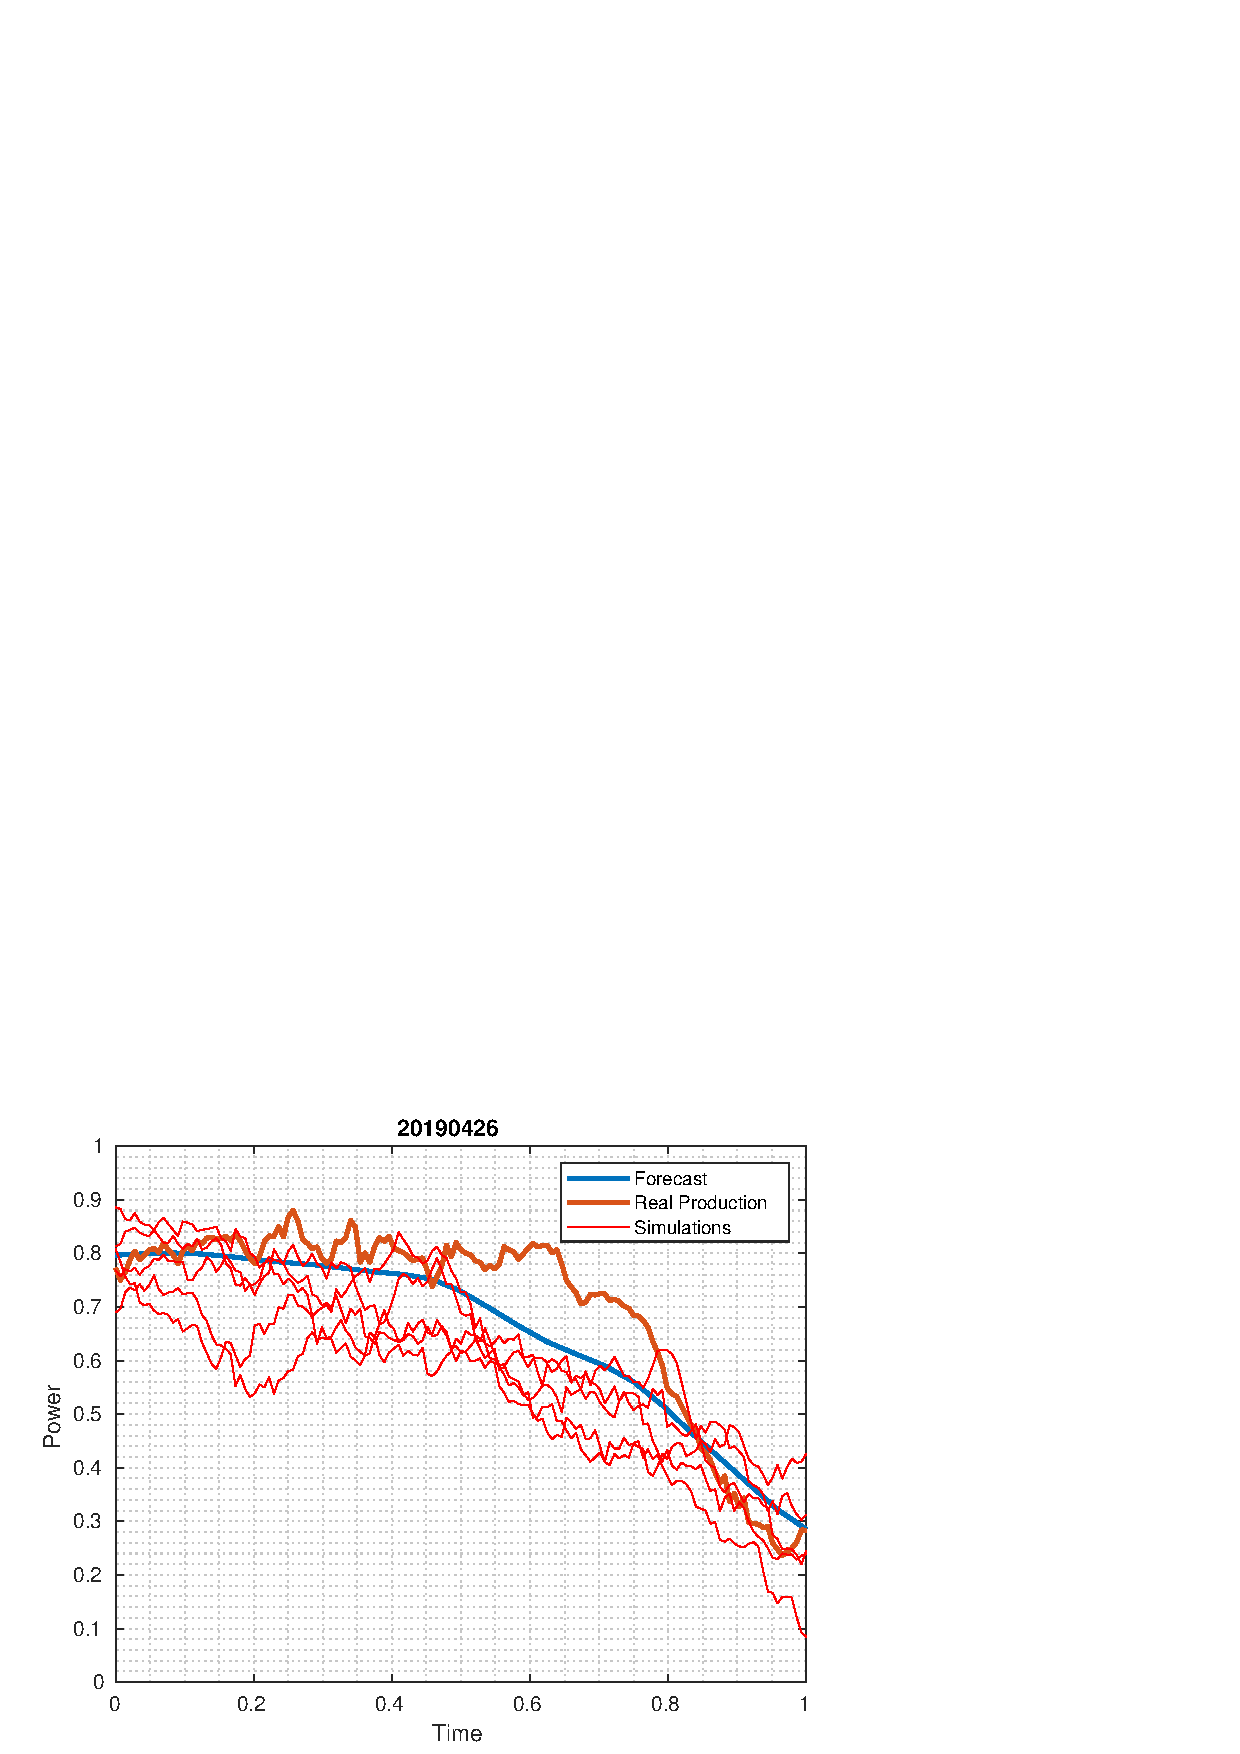
\includegraphics[width=0.9\columnwidth]{2.jpg}

\end{columns}

\end{frame}

\end{document}